\documentclass[conference,a4paper]{IEEEtran}
\IEEEoverridecommandlockouts
\usepackage[T1]{fontenc}
\usepackage{newtxtext,newtxmath}
\usepackage{cite}
\usepackage{amsmath}
\usepackage{graphicx}
\usepackage{booktabs}
\usepackage{array}
\renewcommand\IEEEkeywordsname{Keywords}
\setlength{\tabcolsep}{3pt}

\begin{document}

\title{Cost and Safety of Label Acquisition Strategies for\\
MALDI-TOF Antimicrobial Resistance Prediction}

\author{\IEEEauthorblockN{Muhammad Dyen Asif}
\IEEEauthorblockA{\textit{Department of Computer Science} \\
\textit{National University of Computer}\\
\textit{and Emerging Sciences}\\
Islamabad, Pakistan \\
i240608@isb.nu.edu.pk}
\and
\IEEEauthorblockN{Hira Mastoor}
\IEEEauthorblockA{\textit{Department of Computer Science} \\
\textit{National University of Computer}\\
\textit{and Emerging Sciences}\\
Islamabad, Pakistan \\
hira.mastoor@nu.edu.pk}
\and
\IEEEauthorblockN{Maryam Shahbaz}
\IEEEauthorblockA{\textit{Department of Computer Science} \\
\textit{National University of Computer}\\
\textit{and Emerging Sciences}\\
Islamabad, Pakistan \\
maryam.shahbaz@nu.edu.pk}}

\IEEEpubid{\makebox[\columnwidth]{979-8-3195-2818-6/26/\$31.00~\copyright2026 IEEE\hfill}
\hspace{\columnsep}\makebox[\columnwidth]{ }}

\maketitle
\IEEEpubidadjcol

\begin{abstract}
Machine learning (ML) applied to matrix-assisted laser desorption ionization time-of-flight (MALDI-TOF) mass spectra predicts antimicrobial resistance (AMR) in hours rather than the 1 to 3 days that culture based susceptibility testing takes. A deployed model decays as the local population of isolates changes, so it has to be retrained, and every label is a laboratory susceptibility test that someone pays for. Active learning (AL) is the standard answer to an expensive label, yet a 2026 review of 115 ML studies on clinical MALDI-TOF spectra identified none in which the cost of acquiring labels was a variable. We ran 1540 retraining simulations on the Database of Resistance Information on Antimicrobials and MALDI-TOF Mass Spectra (DRIAMS), covering 3 species and antibiotic pairs, 4 hospitals, 5 budgets and 10 seeds per configuration (5 across hospitals). Models were fitted on 2015 and 2016, bought labels during 2017 in 4 rounds, and were tested on 2018. Across 135 paired comparisons no uncertainty, diversity or hybrid rule beat random selection after correction for multiple testing. Little accuracy was available, since the interval between never retraining and retraining on every arriving isolate spans 0.044 to 0.051 of the area under the receiver operating characteristic curve (AUROC). A budget buys cost rather than accuracy, and 400 tests (19\% to 31\% of a year of isolates) recovered 50\% to 77\% of that interval. Uncertainty sampling, the weakest rule by AUROC, cut the resistant isolates reported susceptible during the pool year by 33\% to 73\%.
\end{abstract}

\begin{IEEEkeywords}
antimicrobial resistance, active learning, MALDI-TOF mass spectrometry, model maintenance, explainable machine learning.
\end{IEEEkeywords}

\section{Introduction}

Antimicrobial resistance is among the largest threats to public health, and an estimated 1.27 million deaths were attributable to bacterial AMR in 2019 \cite{r1}. Treatment depends on knowing which drugs still work, which in routine practice means culture based AST, and that takes up to 72 hours. MALDI-TOF mass spectrometry is already present in most clinical microbiology laboratories for species identification, and the spectrum acquired for that purpose can be reused to predict resistance with ML, which reduces the delay from days to hours \cite{r2}.

Such a model does not stay accurate on its own. The population of isolates in a hospital changes, the instrument is serviced or replaced, and the resistance mechanisms in circulation shift. A model trained here on isolates from 2015 and 2016 reached an AUROC of 0.881 under cross validation inside those years for \textit{Escherichia coli} with ceftriaxone, but only 0.824 on isolates from 2018, a drop of 0.057. Keeping the model useful therefore requires periodic retraining, and retraining requires labels. A label here is a susceptibility test with reagent and technician costs rather than an annotation that a person supplies in seconds, and a laboratory willing to fund only a few hundred extra tests in a year has to decide which isolates receive them.

This is the setting AL was designed for \cite{r3}. The arriving isolates are ranked by the model and labels are bought only where they are expected to be most informative, usually near the decision boundary \cite{r10} or spread across the feature space \cite{r11}. AL is well studied in medical imaging and in text, where it is routinely reported to reach a target accuracy with a fraction of the labels. A systematic review published in 2026, which covers 115 studies that apply ML to clinical MALDI-TOF spectra and groups them by task, preprocessing, model family and evaluation, does not identify a single study in which label acquisition cost is a variable \cite{r4}.

We examine that gap directly. The experiments use DRIAMS, a public collection of clinical MALDI-TOF spectra with matched susceptibility results from 4 Swiss hospitals \cite{r2}. The protocol is temporal rather than a random split. A model is fitted on isolates from 2015 and 2016, isolates arriving during 2017 are offered to an acquisition rule in 4 rounds under a fixed budget, and the maintained model is evaluated on isolates from 2018 (Fig.~1), which keeps the test year strictly after every label that was bought.

The contributions are as follows. This is the first evaluation of label acquisition cost for MALDI-TOF resistance prediction. The main result is negative and holds across 135 paired comparisons, in that no acquisition rule outperformed random selection. We account for that result by measuring how little accuracy retraining makes available in the first place, and we report how much of the benefit of retraining a partial test budget recovers (Table~\ref{tab:cost}). Model quality next year and patient exposure this year are then separated, and the two disagree about which rule is preferable (Fig.~3). TreeSHAP finally shows that models trained under different acquisition rules rely on the same spectral regions (Table~\ref{tab:shap}).

\section{Related Work}

\subsection{Resistance prediction from mass spectra}

Resistance prediction from MALDI-TOF spectra became a practical proposition with the release of DRIAMS, which pairs more than 300000 routine spectra with susceptibility results and established that gradient boosted trees and shallow networks reach clinically interesting discrimination on several species and antibiotic combinations \cite{r2}. The representation was later improved with topological and kernel methods \cite{r5}, and statistical guarantees were added through conformal prediction \cite{r7}. SHAP values were used for interpretation in 21 of the 115 studies covered by the review of Schmidt-Santiago \textit{et al.}, so model explanation is established practice on this modality, while temporal evaluation remains uncommon \cite{r4}. Generalisation across hospitals has been studied directly, and performance dropped sharply when a model was moved to a site it was not trained on \cite{r6}.

\subsection{Label acquisition under a budget}

Active learning has a long history. Uncertainty sampling selects the instances closest to the decision boundary \cite{r10}, core set and diversity methods instead cover the input space \cite{r11}, and importance weighted and cost sensitive variants correct the bias that selective querying introduces \cite{r12}, \cite{r13}. Hybrid rules combine the two signals \cite{r14}. The literature is not uniformly positive. Random selection is a stronger baseline than it is often given credit for, and injecting randomness into uncertainty sampling improved its robustness \cite{r15}. In security, where models are retrained continuously against a moving target, label acquisition under budget has been studied in its own right \cite{r9}, \cite{r16}, and work bridging AL and selective prediction shows that the two interact \cite{r8}.

\subsection{Position of this study}

Prior work on MALDI-TOF resistance prediction has not treated the acquisition of labels as a cost, has largely not used temporal splits, and has rarely reported the 2 clinical error types separately. Work on AL under budget, in turn, has not been applied to this modality.

\section{Method}

\subsection{Problem setting}

Let a spectrum be a vector \textit{x} of 6000 binned intensities and let \textit{y} be 1 if the isolate is resistant or intermediate to the antibiotic of interest and 0 if it is susceptible. A model \textit{f} is fitted to the isolates available at the start of the period and outputs an estimated probability of resistance, and a threshold \textit{t} turns that probability into a report (resistant when \textit{f}(\textit{x}) is at least \textit{t}, susceptible otherwise). Isolates then arrive over a year in 4 batches. The model scores every arriving isolate in each round, an acquisition rule selects \textit{B}/4 of them for laboratory testing, where \textit{B} is the budget for the whole year, and the true labels of those isolates are revealed and added to the training set before \textit{f} and \textit{t} are refitted. Isolates that were not selected are reported using the model's own output, which is the operational situation that matters clinically, because those reports reach clinicians without a confirmatory test (Fig.~1).

\begin{figure*}[!t]
\centering
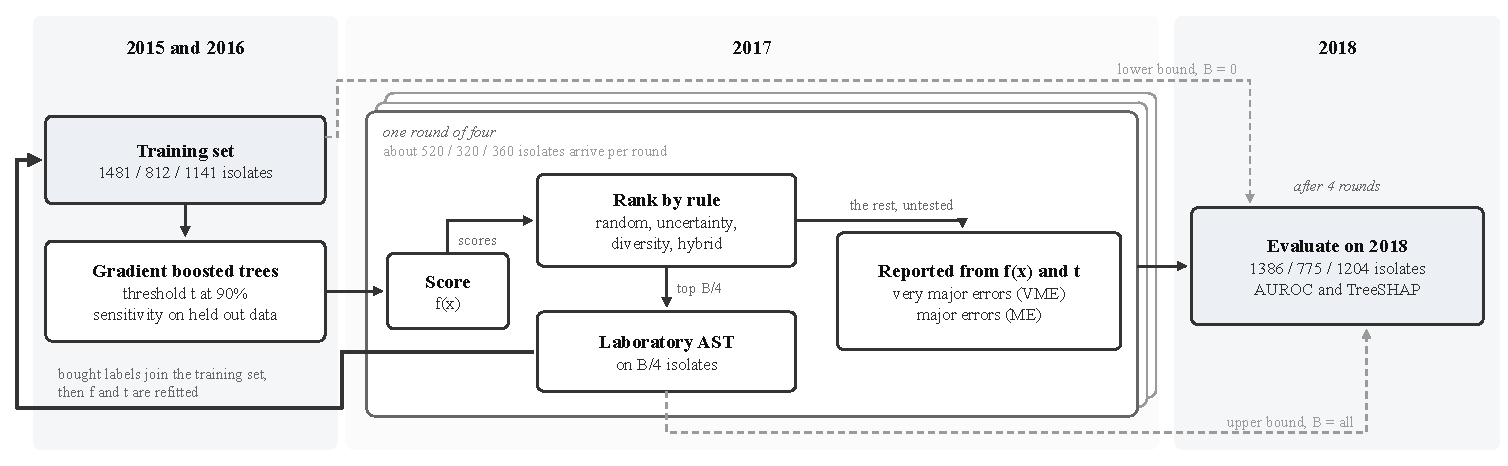
\includegraphics[width=1.0\textwidth]{figures/f1_pipeline.pdf}
\caption{Study pipeline. The 3 counts in each box are the isolates available for \textit{E. coli}, \textit{K. pneumoniae} and \textit{S. aureus} at DRIAMS-A. One of the 4 rounds of 2017 is drawn, in which a quarter of the annual budget B is spent on laboratory susceptibility testing (AST) and those labels enter the training set. Isolates that are not bought are reported from the model output alone, and the dashed arms are the 2 bounds.}
\label{fig:f1_pipeline}
\end{figure*}

\subsection{Acquisition rules}

Four acquisition rules were compared. Random selection draws uniformly from the isolates that arrived in the round and serves as the baseline. Uncertainty sampling takes the isolates whose predicted probability is closest to the threshold \textit{t} \cite{r10}. Diversity sampling applies a \textit{k}-center greedy procedure to the first 50 principal components of the spectra so that the selected isolates are spread out rather than clustered \cite{r11}. The hybrid rule takes the 4\textit{b} isolates closest to the threshold, where \textit{b} is the number bought in the round, and buys one from each of \textit{b} clusters formed by \textit{k}-means \cite{r14}. Two bounds frame all four. The lower bound never retrains at all, and the upper bound retrains on every isolate that arrived, which is what a laboratory would obtain if it tested everything.

\subsection{Error types}

Clinical microbiology distinguishes two kinds of mistake, and they are not interchangeable. A very major error (VME) is a resistant isolate reported as susceptible, which can send a patient home on a drug that will not work. A major error (ME) is a susceptible isolate reported as resistant, which wastes a broader spectrum agent and contributes to selection pressure. The definitions follow the International Organization for Standardization (ISO) standard 20776-2 \cite{r17}. Both are reported throughout, because a rule that lowers one while raising the other has not improved anything.

\subsection{Predictive and operational views}

Two views that are often conflated are kept apart here. The predictive view is the usual one, namely how well next year's model discriminates, measured as AUROC on the 2018 isolates. The operational view counts what happened during the pool year itself, namely how many of the isolates that were not selected for testing were resistant and were nonetheless reported susceptible. These are counts of patients affected rather than rates, and the two views do not have to agree.

\subsection{Explaining the fitted models}

SHAP values were computed to understand why the rules behave similarly \cite{r18}. We used the TreeSHAP implementation inside the gradient boosting library itself \cite{r19}. Six models were explained per pair (the two bounds, and random and uncertainty acquisition at budgets of 400 and 800 labels) on the same 2018 isolates, so any difference is a difference between models rather than between evaluation sets. Two models were then compared by the overlap of their 20 most used bins and by the rank correlation over all 6000 bins. Importance of a bin is its mean absolute SHAP value.

\section{Experimental Setup}

\subsection{Data and splits}

DRIAMS provides spectra preprocessed to 6000 bins of 3 daltons each, spanning 2000 to 20000 daltons. Three species and antibiotic pairs have enough labelled isolates for a temporal analysis and were studied here, namely \textit{E. coli} with ceftriaxone, \textit{Klebsiella pneumoniae} with ceftriaxone, and \textit{Staphylococcus aureus} with oxacillin. At the primary site (DRIAMS-A) these gave 1481, 812 and 1141 training isolates from 2015 and 2016, pools of 2094, 1273 and 1445 isolates arriving in 2017, and test sets of 1386, 775 and 1204 isolates from 2018, with resistance prevalence in the test year of 18.5\%, 13.9\% and 14.6\% respectively. The released spectra carry no acquisition dates, so the 4 arrival batches were formed by a deterministic hash of the isolate code rather than by calendar quarter (the MD5 digest of the code modulo 4). The batches decide which isolates compete for the budget of a round, but their order carries no calendar information. The cross site experiment moves a model trained at DRIAMS-A to each of DRIAMS-B, DRIAMS-C and DRIAMS-D. The source model was fitted on the DRIAMS-A isolates of 2015 to 2018. The 2018 isolates of the target site were divided in half, stratified by label and redrawn for every seed, into a pool and a test set. The budget (25 to 400 labels) was spent in a single round, and the model was refitted on the source isolates together with the bought ones. \textit{S. aureus} with oxacillin has no labelled isolates at DRIAMS-D, which leaves 8 combinations of pair and site.

\subsection{Model and protocol}

The classifier is a gradient boosted tree ensemble \cite{r19}, tuned once on the 2015 and 2016 data only and then held fixed, so that no information from the pool or test years entered the configuration. Of the training years, 20\% was held out to set the threshold \textit{t} at the highest value that still gave 90\% sensitivity to resistance, which reflects the clinical preference for avoiding very major errors. Budgets of 40, 100, 200, 400 and 800 labels were spread evenly over the 4 rounds. Every configuration was repeated with 10 random seeds, and the cross site configurations with 5, giving 1540 retraining simulations in total (660 temporal and 880 cross site).

\subsection{Statistics and availability}

Each rule was compared with random selection on matched seeds using the exact two sided Wilcoxon signed rank test on the paired difference in test AUROC. The resulting p values were corrected with the Holm procedure \cite{r20}, both within each species and antibiotic pair (15 comparisons) and across all 45 temporal comparisons. With 10 seeds no value can fall below 0.002 before correction, 0.029 after correction within a pair or 0.088 across all 45, and with the 5 seeds of the cross site setting no test can reach 0.05. Every comparison is therefore also given as the mean paired difference with its 95\% confidence interval (Table~\ref{tab:effects}). The DRIAMS release used here is archived at doi:10.5061/\allowbreak dryad.\allowbreak bzkh1899q, and our code, the per isolate acquisition log and the per run result records are released with the paper.

\section{Results}

\subsection{Bounds on the available gain}

Two bounds define the space in which any acquisition rule has to operate. A model that was never retrained reached an AUROC on the 2018 isolates of 0.823, 0.742 and 0.799 for the 3 pairs, while a model retrained on every isolate that arrived in 2017 reached 0.867, 0.788 and 0.850. The difference between the 2 bounds was 0.044 (\textit{E. coli}), 0.046 (\textit{K. pneumoniae}) and 0.051 (\textit{S. aureus}) of AUROC, so every acquisition rule competes inside a window of about 5 points, and the standard error over 10 seeds was of a similar order at the smaller budgets (Fig.~2).

\begin{figure*}[!t]
\centering
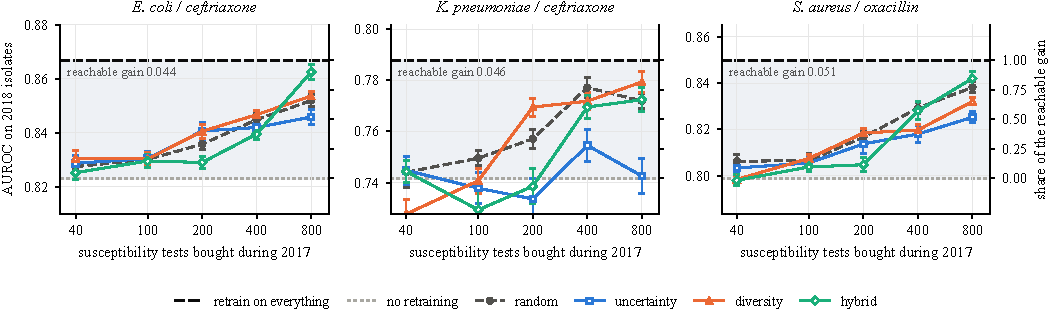
\includegraphics[width=1.0\textwidth]{figures/f2_curves.pdf}
\caption{Test AUROC on 2018 isolates against the number of susceptibility tests bought during 2017, for each species and antibiotic pair. Points are means over 10 seeds and bars are standard errors. The shaded band runs from never retraining (dotted line) to retraining on every arriving isolate (dashed line), and its height is printed inside each panel. The right hand axis reads the same band as a share of the gain retraining makes available. All 4 rules lie inside the band and their intervals overlap at almost every budget.}
\label{fig:f2_curves}
\end{figure*}

\subsection{Comparison against random selection}

All 4 rules improved with budget and all of them stayed between the 2 bounds, but they were not separable from one another (Fig.~2). The temporal setting gives 45 comparisons against random selection (3 pairs, 5 budgets and 3 competing rules), of which 14 reached $p < 0.05$ before correction (12 against the rule and 2 for it, as Table~\ref{tab:effects} shows) and 2 survived the Holm procedure within their pair, both of them in favour of random selection. Uncertainty sampling on \textit{K. pneumoniae} at 800 labels was worse by 0.029 AUROC (95\% confidence interval 0.014 to 0.045) and diversity sampling on \textit{S. aureus} at 40 labels was worse by 0.008 (0.003 to 0.013), each at $p = 0.029$. Corrected across all 45 instead, no comparison stays below 0.05 (smallest 0.088). The cross site experiment adds 120 further comparisons, but in 30 of them the budget was at least as large as the pool of the target site, so every rule bought the same isolates. Of the other 90 the mean difference was negative in 64, and its interval excluded zero in 7, 6 against the rule and 1 for it. These 135 paired comparisons produce no evidence that an informed rule helps, and the differences that can be detected mostly favour random selection.

\begin{table}[!t]
\caption{Mean paired AUROC difference ($\times$100) between each rule and random selection on the 2018 isolates, $\pm$ the half width of its 95\% confidence interval (10 seeds). A dagger marks an interval excluding zero, before correction.}
\label{tab:effects}
\centering\scriptsize
\setlength{\tabcolsep}{1.6pt}
\begin{tabular}{@{}llrrrrr@{}}
\toprule
\textit{Pair} & \textit{Rule} & \textit{40} & \textit{100} & \textit{200} & \textit{400} & \textit{800} \\
\midrule
\textit{E. coli} & Unc. & 0.1$\pm$0.9 & 0.0$\pm$0.9 & 0.5$\pm$1.0 & $-$0.3$\pm$0.7 & $-$0.6$\pm$1.0 \\
 & Div. & 0.3$\pm$0.8 & 0.0$\pm$0.9 & 0.5$\pm$0.7 & 0.2$\pm$0.8 & 0.2$\pm$0.6 \\
 & Hyb. & $-$0.2$\pm$0.9 & $-$0.1$\pm$0.8 & $-$0.7$\pm$0.8 & $-$0.5$\pm$0.7 & 1.1$^{\dagger}$$\pm$0.6 \\
\midrule
\textit{K. pneu.} & Unc. & 0.1$\pm$1.0 & $-$1.2$\pm$1.7 & $-$2.3$^{\dagger}$$\pm$1.6 & $-$2.3$^{\dagger}$$\pm$1.7 & $-$2.9$^{\dagger}$$\pm$1.5 \\
 & Div. & $-$1.6$^{\dagger}$$\pm$1.6 & $-$0.9$\pm$1.0 & 1.2$^{\dagger}$$\pm$0.8 & $-$0.5$\pm$1.4 & 0.7$\pm$0.9 \\
 & Hyb. & 0.0$\pm$1.1 & $-$2.0$\pm$2.2 & $-$1.9$^{\dagger}$$\pm$1.7 & $-$0.8$\pm$1.3 & 0.0$\pm$1.0 \\
\midrule
\textit{S. aureus} & Unc. & $-$0.3$\pm$0.7 & $-$0.1$\pm$1.0 & $-$0.3$\pm$0.9 & $-$1.1$^{\dagger}$$\pm$0.9 & $-$1.3$^{\dagger}$$\pm$0.8 \\
 & Div. & $-$0.8$^{\dagger}$$\pm$0.5 & 0.1$\pm$0.6 & 0.2$\pm$0.6 & $-$1.0$^{\dagger}$$\pm$0.6 & $-$0.6$^{\dagger}$$\pm$0.5 \\
 & Hyb. & $-$0.8$^{\dagger}$$\pm$0.6 & $-$0.3$\pm$0.8 & $-$1.2$^{\dagger}$$\pm$0.9 & $-$0.1$\pm$0.8 & 0.4$\pm$0.7 \\
\bottomrule
\end{tabular}
\end{table}


Because the batches are a pseudo ordering, the comparison at 100, 400 and 800 labels was repeated with 3 further divisions of the 2017 pool drawn from independent hashes and once with the whole budget bought in a single round. A rerun of the original division reproduced all 360 published runs exactly. After correction within each pair, 8 comparisons across the 5 divisions favoured random selection and 1 favoured a rule (diversity sampling on \textit{K. pneumoniae} at 800 labels, better by 0.025, 0.014 to 0.036, and positive in every division). Uncertainty sampling at 800 labels reduced the resistant isolates reported susceptible in every division and for every pair.

\begin{figure*}[!t]
\centering
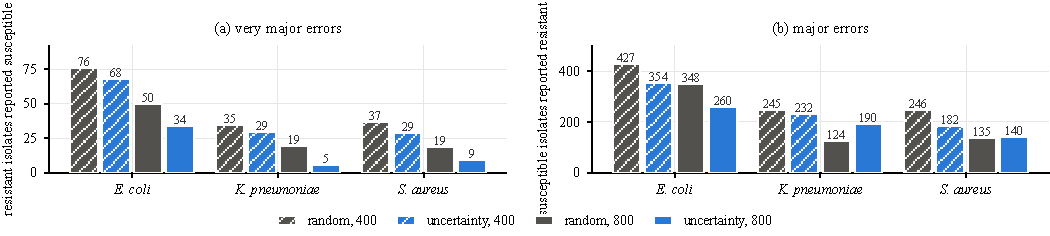
\includegraphics[width=1.0\textwidth]{figures/f3_errors.pdf}
\caption{Clinical errors on the isolates that were not selected for testing, summed over the pool year and averaged over 10 seeds. Hatched bars are a budget of 400 tests and solid bars 800. Panel (a) counts resistant isolates that would have been reported susceptible, panel (b) susceptible isolates that would have been reported resistant.}
\label{fig:f3_errors}
\end{figure*}

\subsection{Cost of a partial test budget}

\begin{table}[!t]
\caption{Share of the available AUROC gain recovered at each budget, averaged over 10 seeds. A value of 1.00 would match retraining on every isolate and 0.00 would match never retraining. }
\label{tab:cost}
\centering\footnotesize
\setlength{\tabcolsep}{2.3pt}
\begin{tabular}{@{}lrrrrrrr@{}}
\toprule
\textit{Pair} & \textit{\shortstack[r]{Tests\\bought}} & \textit{Of pool} & \textit{\shortstack[r]{Tests\\saved}} & \textit{Random} & \textit{Uncert.} & \textit{Divers.} & \textit{Hybrid} \\
\midrule
\textit{E. coli} & 400 & 2094 & 80.9\% & 0.50 & 0.43 & 0.54 & 0.38 \\
 & 800 & 2094 & 61.8\% & 0.66 & 0.52 & 0.70 & 0.90 \\
\midrule
\textit{K. pneumoniae} & 400 & 1273 & 68.6\% & 0.77 & 0.28 & 0.65 & 0.60 \\
 & 800 & 1273 & 37.2\% & 0.66 & 0.02 & 0.82 & 0.67 \\
\midrule
\textit{S. aureus} & 400 & 1445 & 72.3\% & 0.60 & 0.38 & 0.41 & 0.57 \\
 & 800 & 1445 & 44.6\% & 0.77 & 0.52 & 0.65 & 0.85 \\
\bottomrule
\end{tabular}
\end{table}

If the rules are interchangeable, the question worth asking is how many tests to buy rather than which rule to use. Testing every isolate that arrives in a year costs 2094, 1273 and 1445 susceptibility tests at DRIAMS-A, and a budget of 400 tests (19\% to 31\% of those totals) recovered about half of the available gain for \textit{E. coli} (0.50) and roughly three quarters for \textit{K. pneumoniae} (0.77), which is what Table~\ref{tab:cost} expresses as a price. The curve of benefit against labels is steep at the start and flat later (Fig.~2), so most of the value lies in the decision to retrain at all, and comparatively little in the decision about which isolates to retrain on.

\subsection{Operational errors during the pool year}


AUROC describes next year's model and says nothing about the patients whose isolates were reported during the year in which the labels were being collected, which is what Fig.~3 counts. At a budget of 800 tests the number of resistant isolates that went untested and would have been reported susceptible fell from 49.8 to 33.6 for \textit{E. coli} under uncertainty sampling rather than random selection, from 19.4 to 5.2 for \textit{K. pneumoniae}, and from 18.8 to 9.2 for \textit{S. aureus}, reductions of 33\%, 73\% and 51\%. Major errors moved in the same direction for 2 of the 3 pairs, falling from 347.8 to 259.8 for \textit{E. coli} and staying level for \textit{S. aureus} (134.6 to 140.0), but they rose from 123.7 to 190.1 for \textit{K. pneumoniae}, which is the one configuration in which the safety gain is paid for in broad spectrum prescribing.

The mechanism is visible in the acquisition log, which records one line per isolate per round. Uncertainty sampling bought fewer resistant isolates than random selection did. The resistant share of what it bought at a budget of 400 labels was 14.9\%, 9.7\% and 10.8\%, against arrival rates of 22.2\%, 14.2\% and 18.8\%. An isolate that the model confidently calls resistant lies far from the threshold, so the rule declines to pay for it, and the isolates it does buy sit 2 to 4 times closer to the threshold (median absolute distance 0.008 against 0.030 for \textit{E. coli}) than those it skips. Uncertainty sampling is therefore a detector of impending mistakes rather than a detector of resistance.

\subsection{SHAP profiles of the fitted models}

Models that differ only in how their labels were chosen agreed with each other about as much as either agreed with the model retrained on everything (Table~\ref{tab:shap}). The model that was never retrained was the outlier in every pair, and on \textit{K. pneumoniae} it shared only 2 of 20 bins with the fully retrained model (Jaccard index 0.11, $\rho$ = 0.22). Retraining changes what a model looks at, whereas changing the acquisition rule at a fixed amount of retraining largely does not.

\begin{table}[!t]
\caption{Agreement between fitted models in their SHAP profiles. J is the Jaccard overlap of the 20 most used spectral bins. $\rho$ is the Spearman rank correlation of importance over all 6000 bins.}
\label{tab:shap}
\centering\footnotesize
\begin{tabular}{@{}lrrrrrr@{}}
\toprule
 & \multicolumn{2}{c}{\textit{E. coli}} & \multicolumn{2}{c}{\textit{K. pneu.}} & \multicolumn{2}{c}{\textit{S. aureus}} \\
\cmidrule(lr){2-3}\cmidrule(lr){4-5}\cmidrule(l){6-7}
\textit{Models compared} & \textit{J} & $\rho$ & \textit{J} & $\rho$ & \textit{J} & $\rho$ \\
\midrule
Random 400 vs uncertainty 400 & 0.60 & 0.38 & 0.38 & 0.44 & 0.54 & 0.44 \\
Random 800 vs uncertainty 800 & 0.60 & 0.39 & 0.29 & 0.44 & 0.43 & 0.48 \\
\midrule
Random 800 vs retrain on all & 0.67 & 0.40 & 0.38 & 0.52 & 0.60 & 0.54 \\
Uncertainty 800 vs retrain on all & 0.60 & 0.39 & 0.38 & 0.48 & 0.43 & 0.47 \\
\midrule
No retraining vs retrain on all & 0.43 & 0.24 & 0.11 & 0.22 & 0.29 & 0.30 \\
Mean over all 15 model pairs & 0.60 & 0.36 & 0.31 & 0.40 & 0.49 & 0.44 \\
\bottomrule
\end{tabular}
\end{table}

Counting how many of the 6 models placed a given bin in their top 20 makes the structure clearer. Nine bins appeared in all 6 lists for \textit{E. coli}, out of 32 that appeared anywhere, and the strongest lay at 2150 to 2156 daltons. The figure was 8 of 40 for \textit{S. aureus}, at 2405 to 2411 and 2852 to 2858 daltons, and only 2 of 57 for \textit{K. pneumoniae}, which matches that pair having the fewest isolates, the lowest AUROC and the least stable explanations.

\section{Discussion}

\subsection{Why label efficiency is the wrong objective here}

The natural reading of a negative result is that the method was implemented badly. The better reading here is that label efficiency is the wrong objective for this problem. AL promises to reach a given accuracy with fewer labels, and that promise is only valuable when the accuracy at stake is large. On this modality the entire gap between never retraining and retraining on everything is around 5 points of AUROC (0.044 to 0.051), and the training years already contain thousands of examples of the few spectral peaks that carry the signal. One more year of isolates adds mostly repetition, and choosing which repetitions to buy is a small lever on a problem whose bottleneck lies elsewhere.

\subsection{What a laboratory should take from this}

The acquisition rule still matters, although for a different reason. The rules differ in which patients are exposed to an error while the labels are being gathered, and that difference is large where the accuracy difference is small. A budget of a few hundred tests selected by uncertainty is a reasonable default on these data, since it costs the least, it gives up little AUROC against random selection (0.017 on average over the budgets for \textit{K. pneumoniae}, 0.006 for \textit{S. aureus} and nothing measurable for \textit{E. coli}), and it substantially reduces the resistant isolates that would otherwise be reported susceptible. The \textit{K. pneumoniae} result at 800 labels is the caveat, both because it is the configuration where uncertainty sampling lost the most AUROC and because it is the one where major errors rose (Fig.~3), and a laboratory working on that organism would be buying a 73\% reduction in very major errors at the price of 66 additional major errors over the year. A major error lasts only until the culture based result arrives, so about 5 additional major errors for each very major error avoided is a trade that a laboratory may accept, but it is a trade rather than a free gain. On the 2018 isolates the models maintained by uncertainty sampling also made more very major errors and fewer major errors than those maintained by random selection in 14 of the 15 configurations, so a laboratory adopting the rule should set \textit{t} again on recent labels.

\subsection{Limitations}

The released spectra carry no acquisition dates, so the arrival batches within 2017 are a deterministic pseudo ordering rather than true calendar quarters, although the year boundaries themselves are real. The simulation therefore represents drift between years but not within a year, and a rule that adapts to recent isolates could gain from a real ordering in a way these experiments cannot show. The 3 pairs studied are those with enough labelled isolates for a temporal analysis, and the conclusions may not transfer to rarer organisms or to antibiotics with very low resistance prevalence. \textit{S. aureus} with oxacillin has almost no resistant isolates at 2 of the 4 hospitals, which limits the power of the cross site comparisons for that pair. The explanations were computed from 1 seed per configuration, so some of the disagreement in the tail of the ranking is sampling noise. All of this is a retrospective simulation on stored spectra, in which a bought label is available at once, and the safety result needs confirmation on isolates collected in real time before it is used to set a testing policy. Beyond that, a prospective study would have to contend with laboratory turnaround, with clinicians who may override the model, and with instrument changes that our protocol holds fixed.

\section{Conclusion}

Across 135 paired comparisons spanning 3 species and antibiotic pairs, 4 hospitals and 5 budgets, no uncertainty, diversity or hybrid rule outperformed random selection. The explanation is that retraining makes only 0.044 to 0.051 of AUROC available in total, and that models trained under different rules rely on the same small set of spectral bins (Table~\ref{tab:shap}). The quantity worth reporting is therefore cost rather than label efficiency, in that roughly a third of a year of susceptibility tests recovers between half and three quarters of the benefit of testing everything (Table~\ref{tab:cost}). Uncertainty sampling remains worth using for a different reason, since it reduced by a third to three quarters the resistant isolates that were reported susceptible while the labels were being collected. Future work should test whether these conclusions hold prospectively, on isolates with real acquisition dates, and whether acquisition rules that target the clinical error directly, rather than model uncertainty, do better on the operational view.
\section*{Acknowledgment}
An AI assistant (Claude, Anthropic) was used to support the writing of the analysis code and the
recomputation of the statistical tests.

\begin{thebibliography}{20}
\bibitem{r1} Antimicrobial Resistance Collaborators, ``Global burden of bacterial antimicrobial resistance in 2019: a systematic analysis,'' \textit{The Lancet}, vol. 399, no. 10325, pp. 629-655, 2022.
\bibitem{r2} C. Weis \textit{et al.}, ``Direct antimicrobial resistance prediction from clinical MALDI-TOF mass spectra using machine learning,'' \textit{Nature Medicine}, vol. 28, pp. 164-174, 2022.
\bibitem{r3} B. Settles, ``Active learning literature survey,'' Computer Sciences Technical Report 1648, University of Wisconsin-Madison, 2009.
\bibitem{r4} L. Schmidt-Santiago, A. Guerrero-Lopez, C. Sevilla-Salcedo, D. Rodriguez-Temporal, B. Rodriguez-Sanchez, and V. Gomez-Verdejo, ``A systematic review of machine learning on clinical MALDI-TOF MS,'' \textit{Briefings in Bioinformatics}, vol. 27, 2026, doi:10.1093/bib/bbag208.
\bibitem{r5} C. Weis, M. Horn, B. Rieck, A. Cuenod, A. Egli, and K. Borgwardt, ``Topological and kernel-based microbial phenotype prediction from MALDI-TOF mass spectra,'' \textit{Bioinformatics}, vol. 36, no. S1, pp. i30-i38, 2020.
\bibitem{r6} D. Duroux, P. P. Meyer, G. Visona, and N. Beerenwinkel, ``Generalizable machine learning models for rapid antimicrobial resistance prediction in unseen health care settings,'' \textit{GigaScience}, 2026, doi:10.1093/gigascience/giaf156.
\bibitem{r7} N. Corvelo Benz, L. Miranda, D. Chen, J. Sattler, and K. Borgwardt, ``Detecting antimicrobial resistance through MALDI-TOF mass spectrometry with statistical guarantees using conformal prediction,'' in \textit{Research in Computational Molecular Biology (RECOMB)}, Springer, 2025, doi:10.1007/978-3-031-90252-9\_5.
\bibitem{r8} J. Chen, J. Yoon, S. Ebrahimi, S. O. Arik, S. Jha, and T. Pfister, ``ASPEST: bridging the gap between active learning and selective prediction,'' \textit{Transactions on Machine Learning Research}, 2024.
\bibitem{r9} Y. Chen, Z. Ding, and D. Wagner, ``Continuous learning for Android malware detection,'' in \textit{USENIX Security Symposium}, 2023.
\bibitem{r10} D. D. Lewis and W. A. Gale, ``A sequential algorithm for training text classifiers,'' in \textit{ACM SIGIR}, 1994, pp. 3-12.
\bibitem{r11} O. Sener and S. Savarese, ``Active learning for convolutional neural networks: a core set approach,'' in \textit{International Conference on Learning Representations (ICLR)}, 2018.
\bibitem{r12} A. Beygelzimer, S. Dasgupta, and J. Langford, ``Importance weighted active learning,'' in \textit{International Conference on Machine Learning (ICML)}, 2009, pp. 49-56.
\bibitem{r13} A. Krishnamurthy, A. Agarwal, T.-K. Huang, H. Daum\'e III, and J. Langford, ``Active learning for cost-sensitive classification,'' \textit{Journal of Machine Learning Research}, vol. 20, no. 65, pp. 1-50, 2019.
\bibitem{r14} W.-N. Hsu and H.-T. Lin, ``Active learning by learning,'' in \textit{AAAI Conference on Artificial Intelligence}, 2015, pp. 2659-2665.
\bibitem{r15} P.-Y. Lu, C.-L. Li, and H.-T. Lin, ``A more robust baseline for active learning by injecting randomness to uncertainty sampling,'' in \textit{AI and HCI Workshop at ICML}, 2023.
\bibitem{r16} F. Barbero, F. Pendlebury, F. Pierazzi, and L. Cavallaro, ``Transcending Transcend: revisiting malware classification in the presence of concept drift,'' in \textit{IEEE Symposium on Security and Privacy}, 2022, pp. 805-823.
\bibitem{r17} International Organization for Standardization, \textit{ISO 20776-2:2021, Susceptibility testing of infectious agents and evaluation of performance of antimicrobial susceptibility test devices}, 2021.
\bibitem{r18} S. M. Lundberg \textit{et al.}, ``From local explanations to global understanding with explainable AI for trees,'' \textit{Nature Machine Intelligence}, vol. 2, pp. 56-67, 2020.
\bibitem{r19} T. Chen and C. Guestrin, ``XGBoost: a scalable tree boosting system,'' in \textit{ACM SIGKDD}, 2016, pp. 785-794.
\bibitem{r20} S. Holm, ``A simple sequentially rejective multiple test procedure,'' \textit{Scandinavian Journal of Statistics}, vol. 6, pp. 65-70, 1979.
\end{thebibliography}
\end{document}
